\chapter{Photon Identification Optimization}

Photon identification in ATLAS is carried out through applying cuts to 9 shower shape variables that explain the longitudinal and lateral showering development of electromagnetic interaction in the calorimeter. These include variables describing the leakage in the hadronic calorimeter ($R_{had}$, $R_{had_1}$), widths of energy depositions in the \gls{EM} calorimeter ($w_{\eta_2}$, $w_{s3}$), energy ratios of depositions in the \gls{EM} calorimeter ($R_{\eta}$, $R_{\phi}$, $F_{side}$), and the energy difference and ratios of the strips ($\Delta E$, $E_{ratio}$). Two sets of cuts are defined, corresponding to two working points, nominally the \textit{tight} and \textit{loose} menus.

A schematic of all these variables can be found in Figure \ref{fig:ss-vars-schematic}. Additionally, a table describing these variables can be found in Table \ref{tab:ss-vars-table}.

% todo: maybe describe these a bit better https://arxiv.org/pdf/1606.01813.pdf 

In order to account for detector segmentation and differences in upstream material, cuts on these variables are derived in bins of \abseta. The intervals are 0.0, 0.6, 0.8, 1.15, 1.37, 1.52, 1.81, 2.01, 2.37, with a bin defined between each step (e.g. $[0.0,0.6)$, $[0.6,0.8)$, etc.) except over $[1.37,1.52)$ where the transition crack between the \gls{EMB} and \gls{EMEC} lies. 

% todo: make sure inclusivity here is correct

\begin{figure}[!thp]
    \centering
    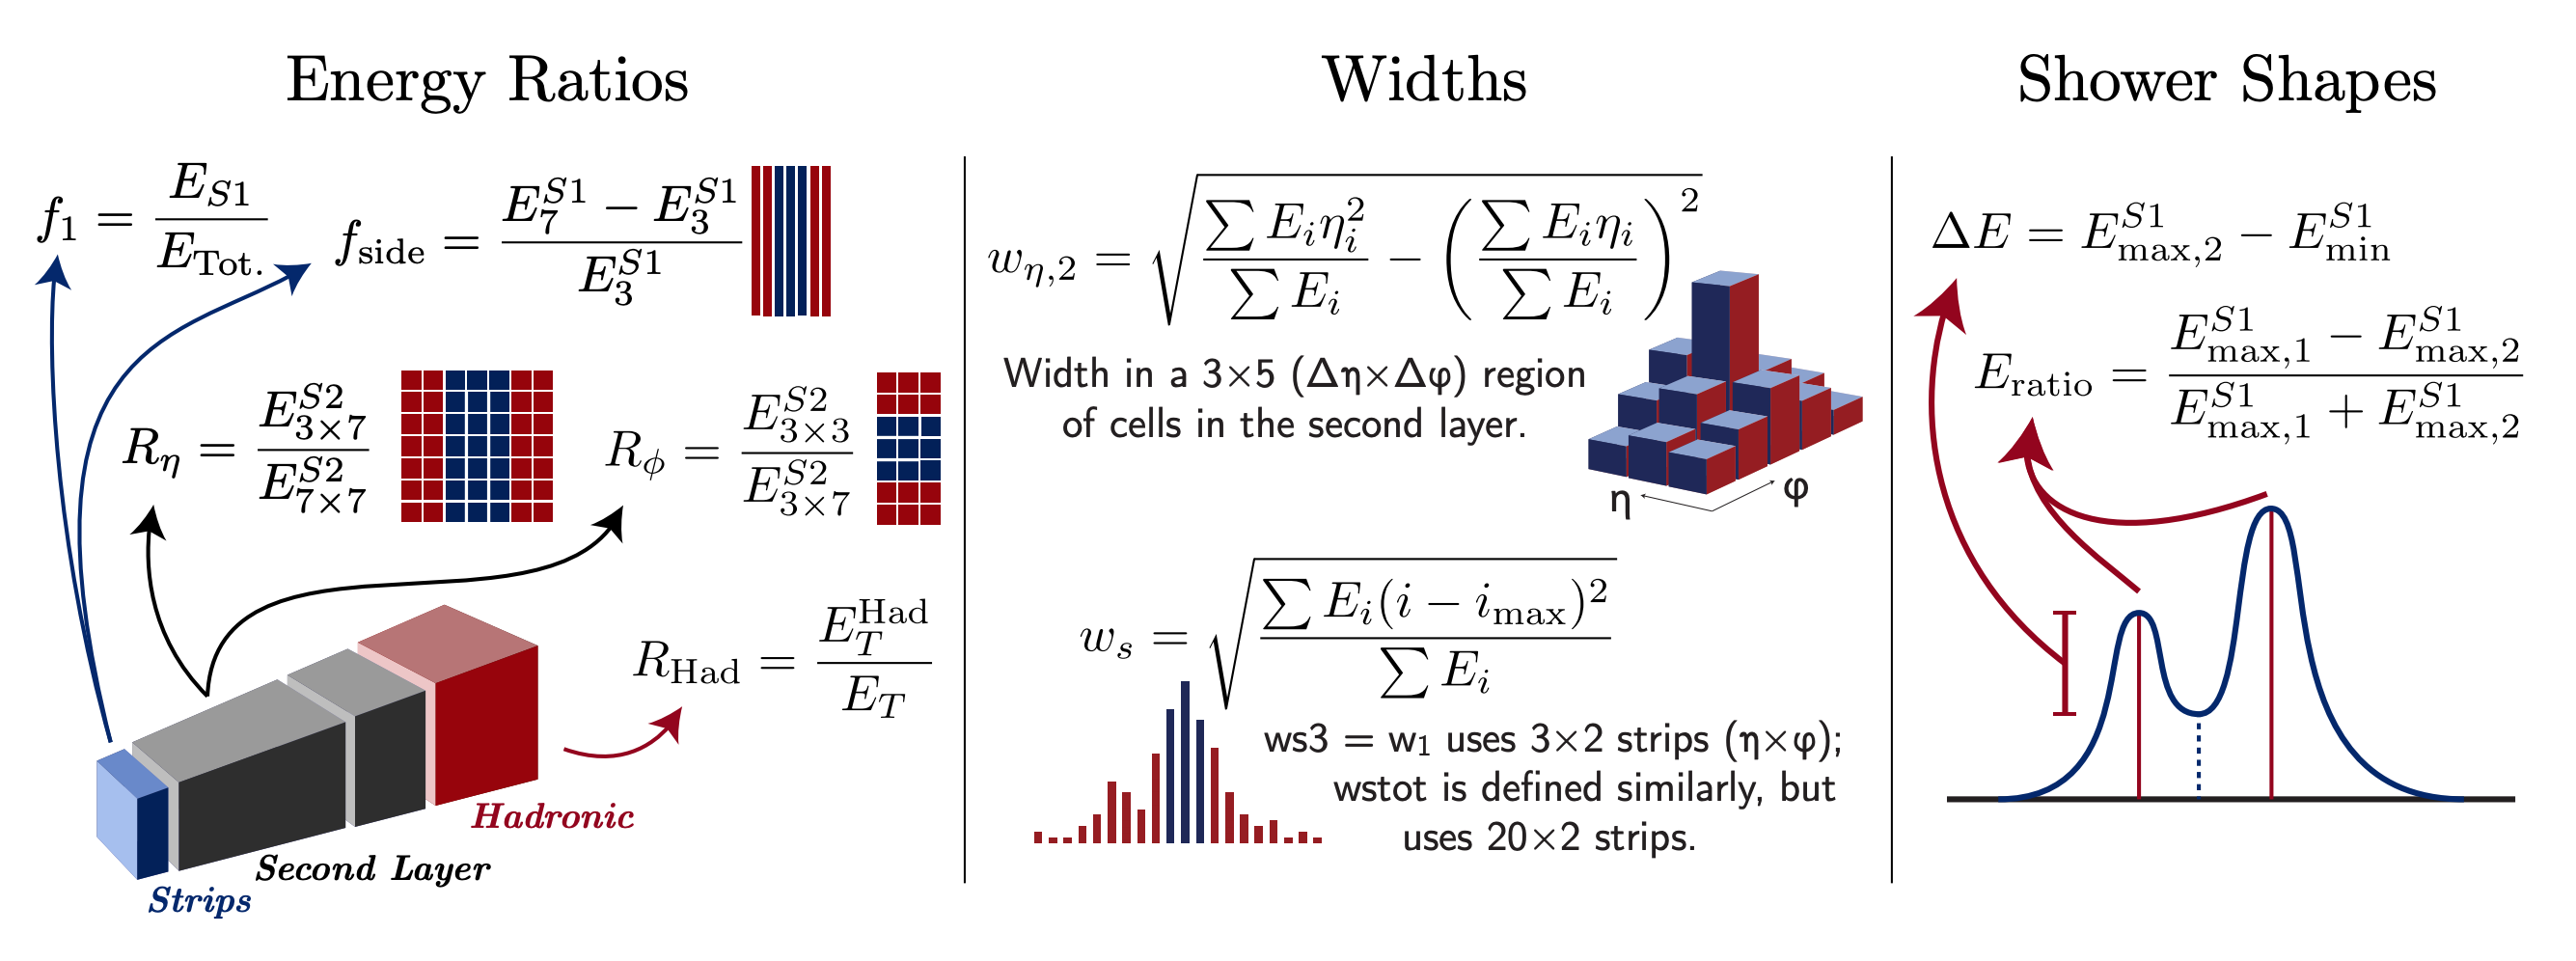
\includegraphics[width=.98\textwidth]{chapters/chapter4_photonID/images/ss-vars.png}
    \caption[Schematic of the shower shape variables used in the present cut-based photon identification menu.]
    {Schematic of the shower shape variables used in the present cut-based photon identification menu \cite{ss-var-schematic}.}
    \label{fig:ss-vars-schematic}
\end{figure}

\begin{table}[!thp]
    \centering
    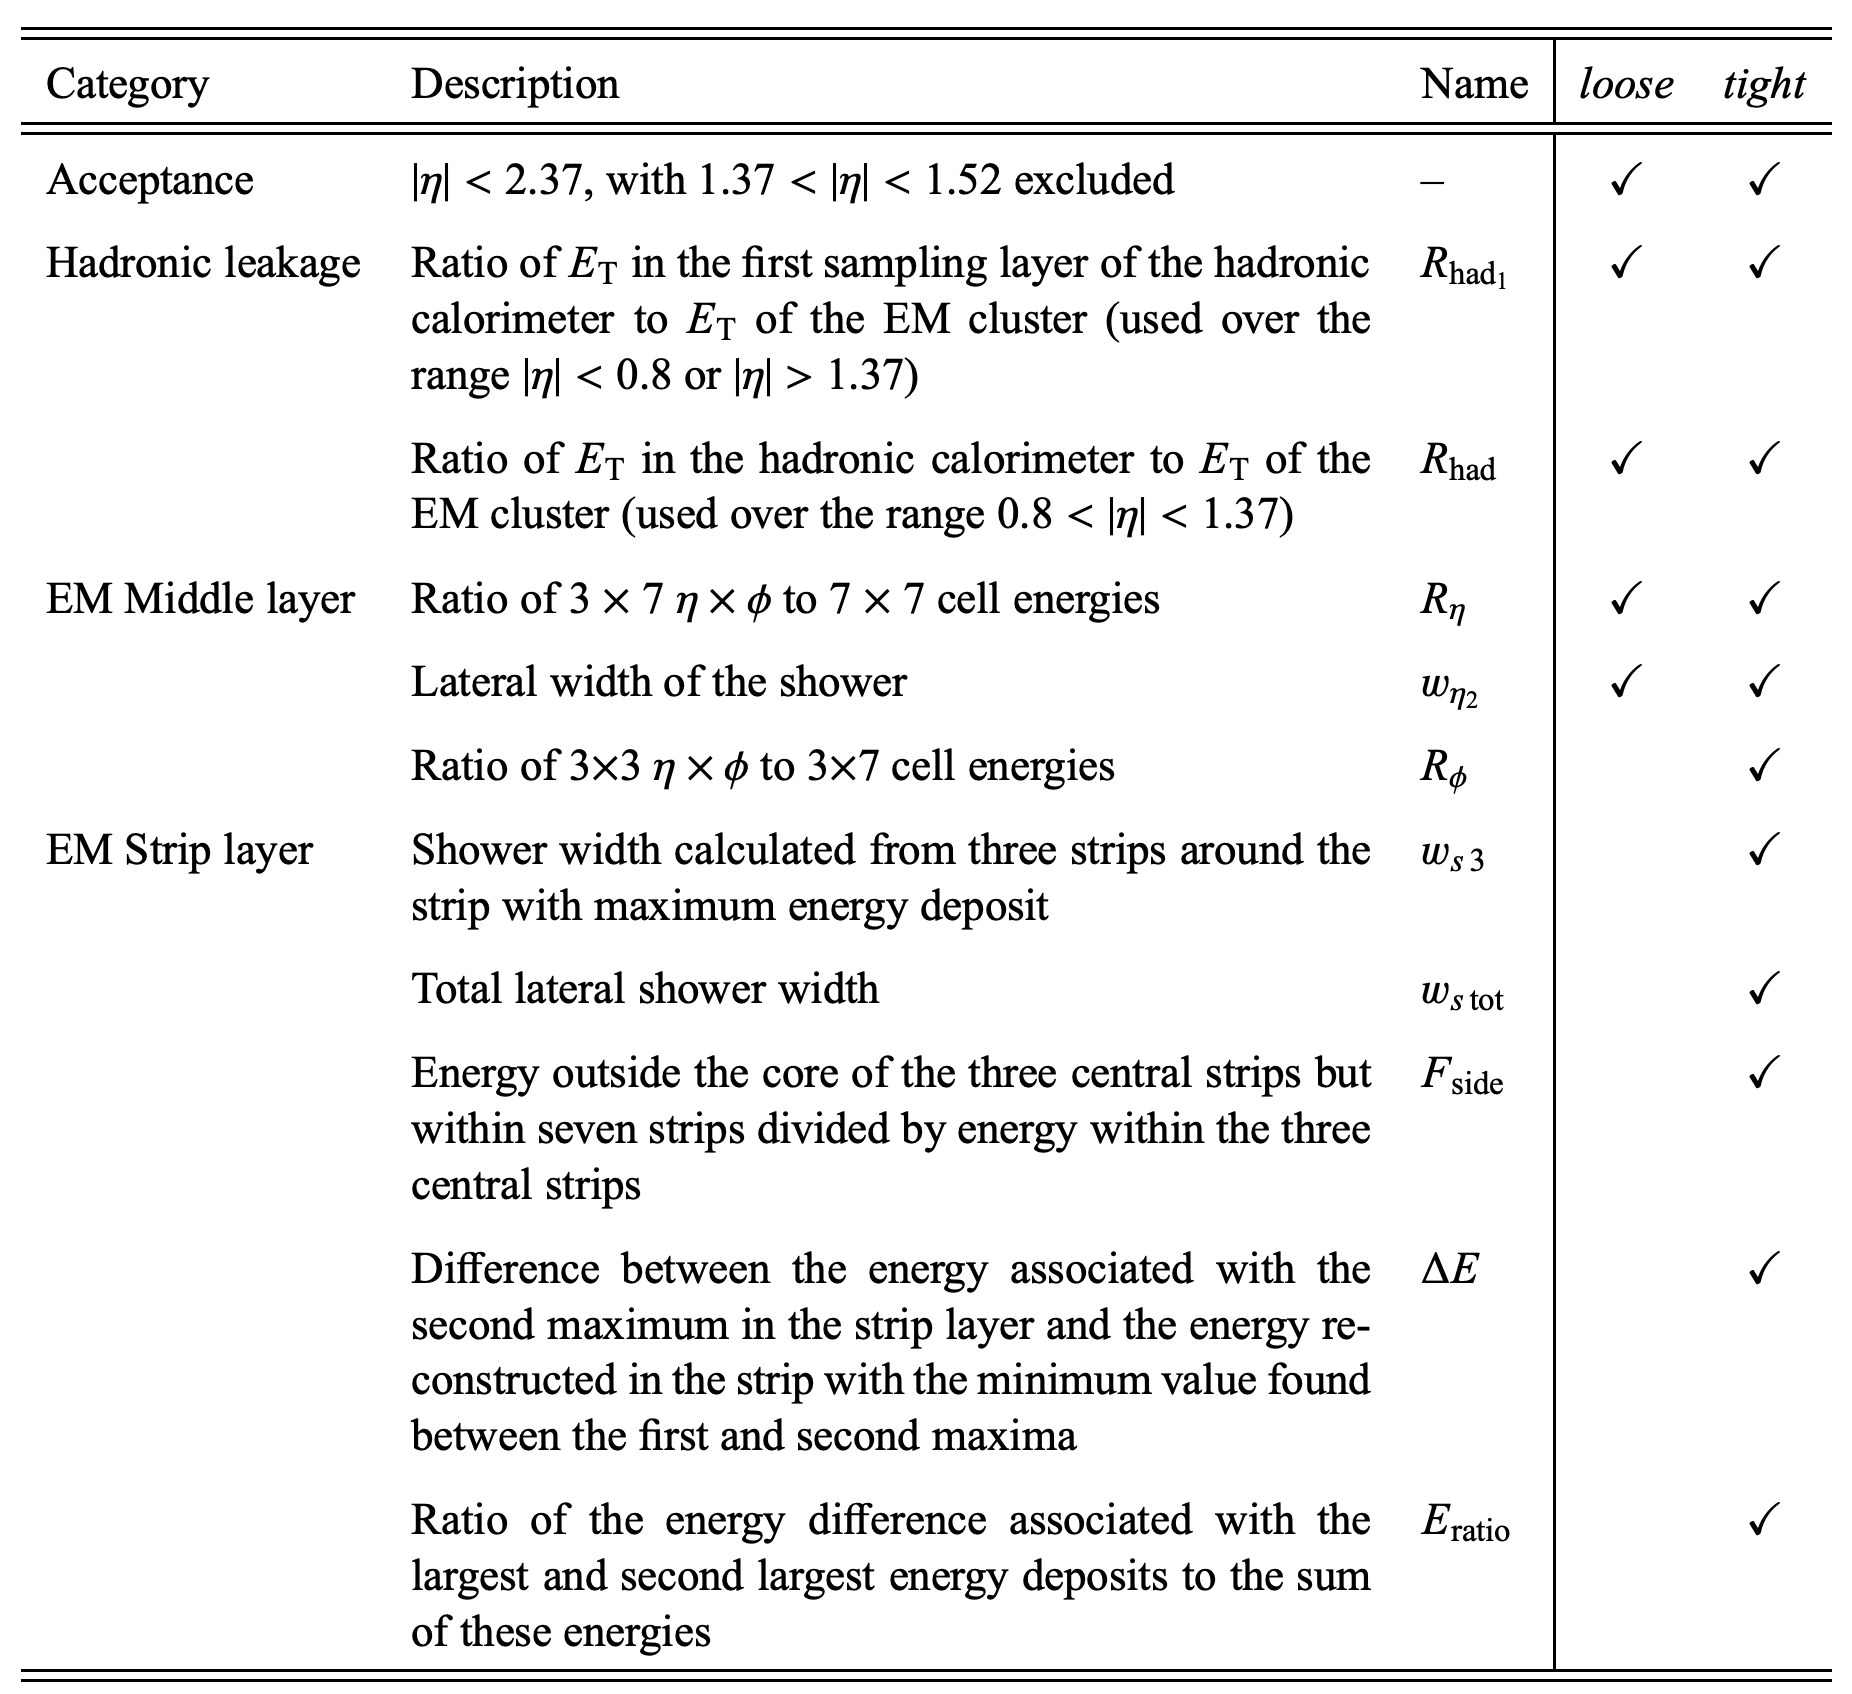
\includegraphics[width=.90\textwidth]{chapters/chapter4_photonID/images/ss-table.png}
    \caption[List of discriminating variables used in the present photon identification menu.]
    {List of discriminating variables used in the present photon identification menu \cite{r1-photonID}.}
    \label{tab:ss-vars-table}
\end{table}

\section{Samples} \label{sec:photon-id-samples}

In optimization of photon identification, the aim is to discriminate prompt photons from various background sources. The predominant background is that from hadronically decaying jets. The signal sample is a $\gamma+$jet sample

Additionally, truth information is used to force 


\section{Topological Clusters}

Photon reconstruction is performed through a method known as ``topological clustering,'' which is outlined in Section \ref{ssec:em-signatures}. In the calorimeter, energy depositions are clustered via this method, then merged into superclusters, which are ultimately the detector signature defined as the photon. The reconstructed observables of these topological clusters, or \textit{moments}, can be used to characterize them. This section will discuss the use of these topological cluster moments in photon identification to better reject background from non-prompt photons.

\noindent\textbf{Shape Information}\\
\indent The size of the topological cell is parametrized by moments in $r_i$ and $\lambda_i$, which are defined as:

\begin{equation}
    r_i = |(\vec{x_i} - \vec{c}) \times \vec{s}| \text{\hspace{2em}(radial distance to shower axis)} \\
\end{equation}
\begin{equation}
    \lambda_i = (\vec{x_i} - \vec{c}) \cdot \vec{s} \text{\hspace{2em}(longitudinal distance to shower center of gravity)} 
\end{equation}

Where $\vec{s}$ is the shower axis and $\vec{c}$ is the center of gravity. Through this parametrization, the topo-cluster can be analyzed as a spheroid, with the second moments in $r$ and $\lambda$ as the extensions. $\sqrt{\langle \lambda^2 \rangle}$ is the semi-major axis in depth (along the shower axis), $\sqrt{\langle r^2 \rangle}$ is the semi-major axis in width.

\noindent\textbf{Location Information}\\
\indent The location of the topo-cluster is calculated from the first moments of the three cartesian coordinates, describing the position of $\vec{c}$. Due to azimuthal symmetry in the detector, the key component to locational parametrization of topo-clusters is the depth in the calorimeter. Thus, this location can be described via $\lambda_{clus}$, the distance of the center of gravity from the front face of the calorimeter.

A visualization of the geometric moments, both location and shape can be found in Figure \ref{fig:topo-geom}, with relevant spacial parameters (i.e. $\vec{c}$, $\vec{s}$, etc) shown and defined.

\begin{figure}[!thp]
    \centering
    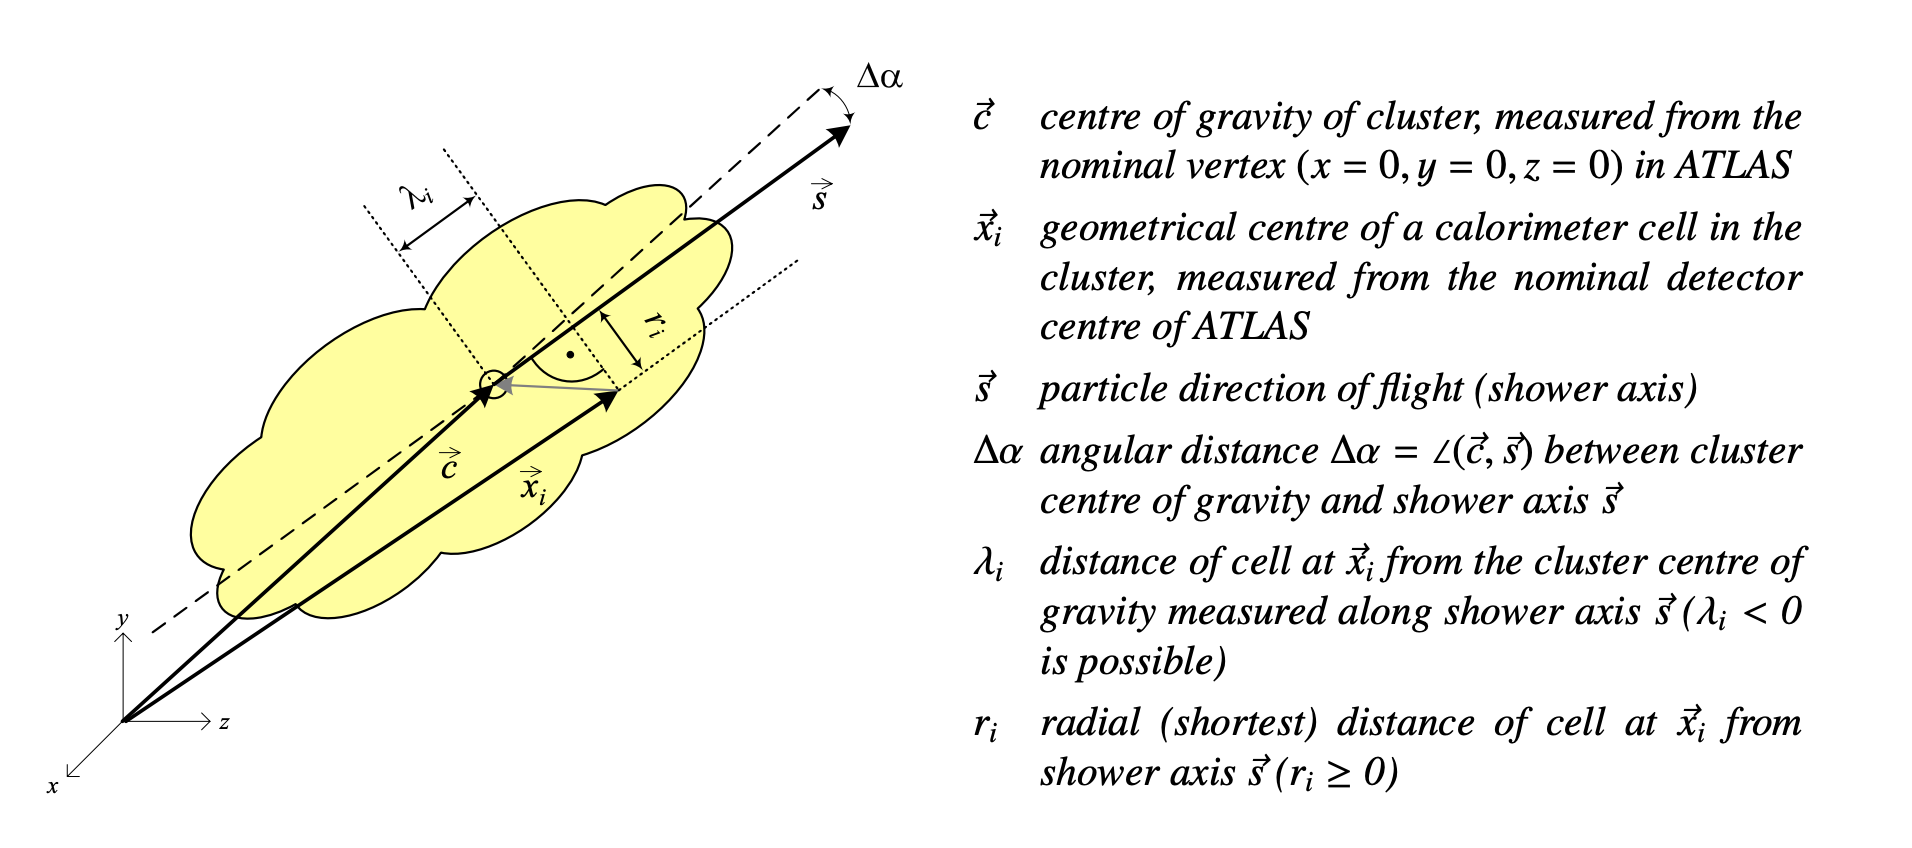
\includegraphics[width=.90\textwidth]{chapters/chapter4_photonID/images/geom-moments.png}

    \caption[The geometric moments and relevant parameters for topo-clusters.]
    {The geometric moments and relevant parameters for topo-clusters \cite{topo-clustering-r1}.}
    \label{fig:topo-geom}
\end{figure}


\subsection{Data-MC Comparison}
In order to ensure that the topological clusters are properly modeled in the \gls{MC}, the variables investigated are compared to data. To do so, the present tight photon ID is applied to both the \gls{MC} and data. Furthermore, photons in \gls{MC} must correspond to a truth photon. 


This section includes the comparisons for unconverted photons which are considered for adding to the photon ID menu. Converted comparisons will be included into Appendix 

% TODO: add appendix

%todo: add plots

\begin{figure}[!thp]
    \centering
    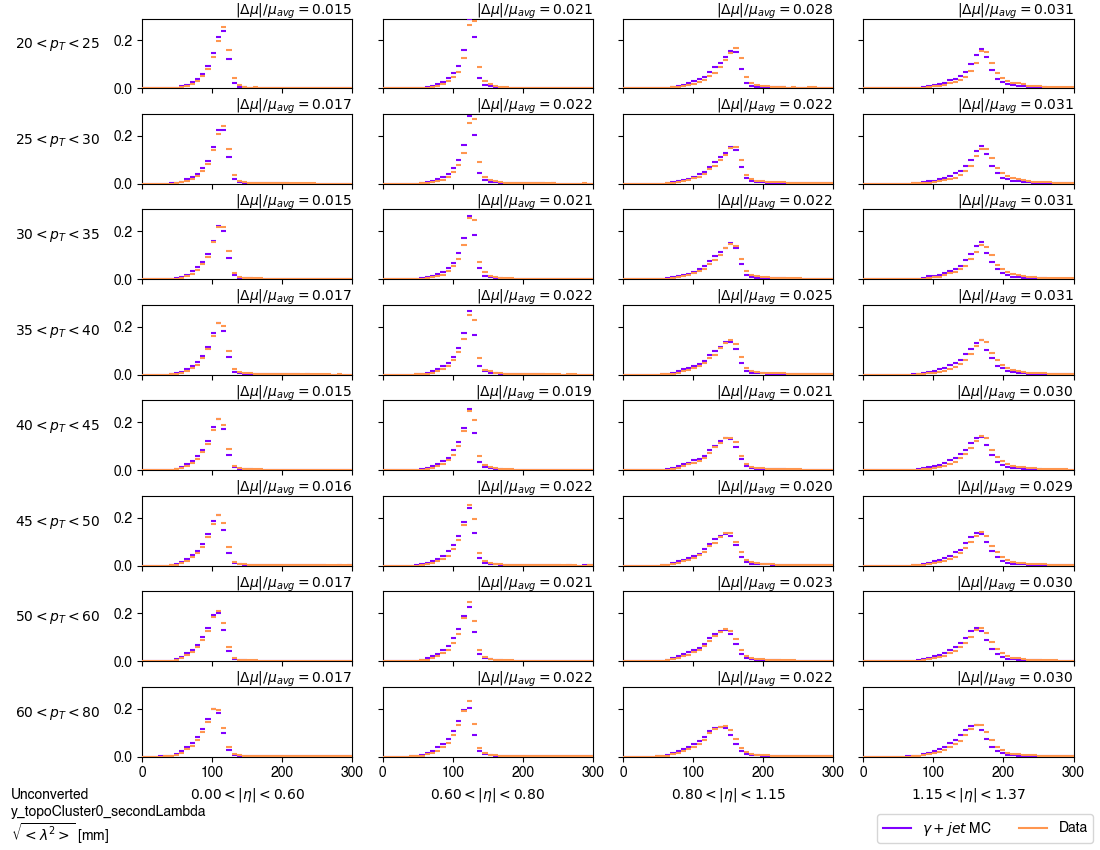
\includegraphics[width=.80\textwidth]{chapters/chapter4_photonID/images/y_topoCluster0_secondLambda_Unconverted_lowerEta.png}
    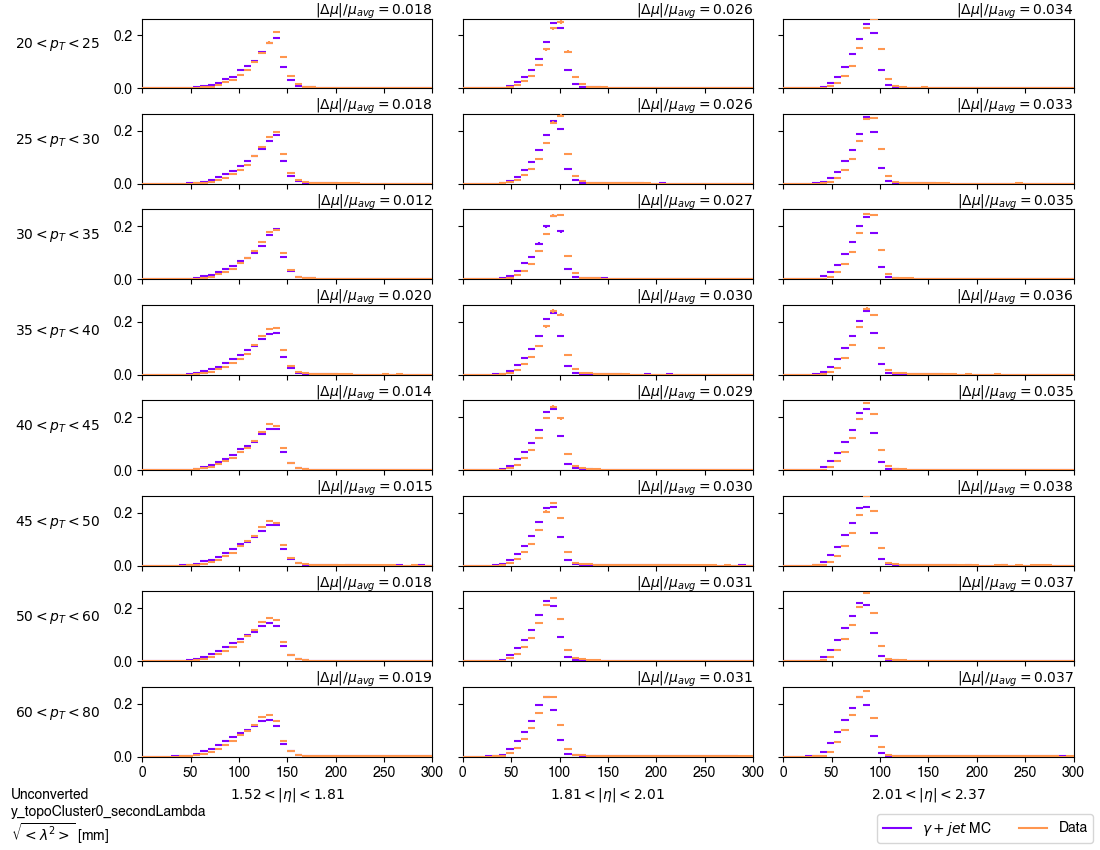
\includegraphics[width=.80\textwidth]{chapters/chapter4_photonID/images/y_topoCluster0_secondLambda_Unconverted_upperEta.png}
    \caption{Data-MC comparison for the semi-major axis in depth ($\sqrt{\lambda^2}$).}
\end{figure}
\begin{figure}[!thp]
    \centering
    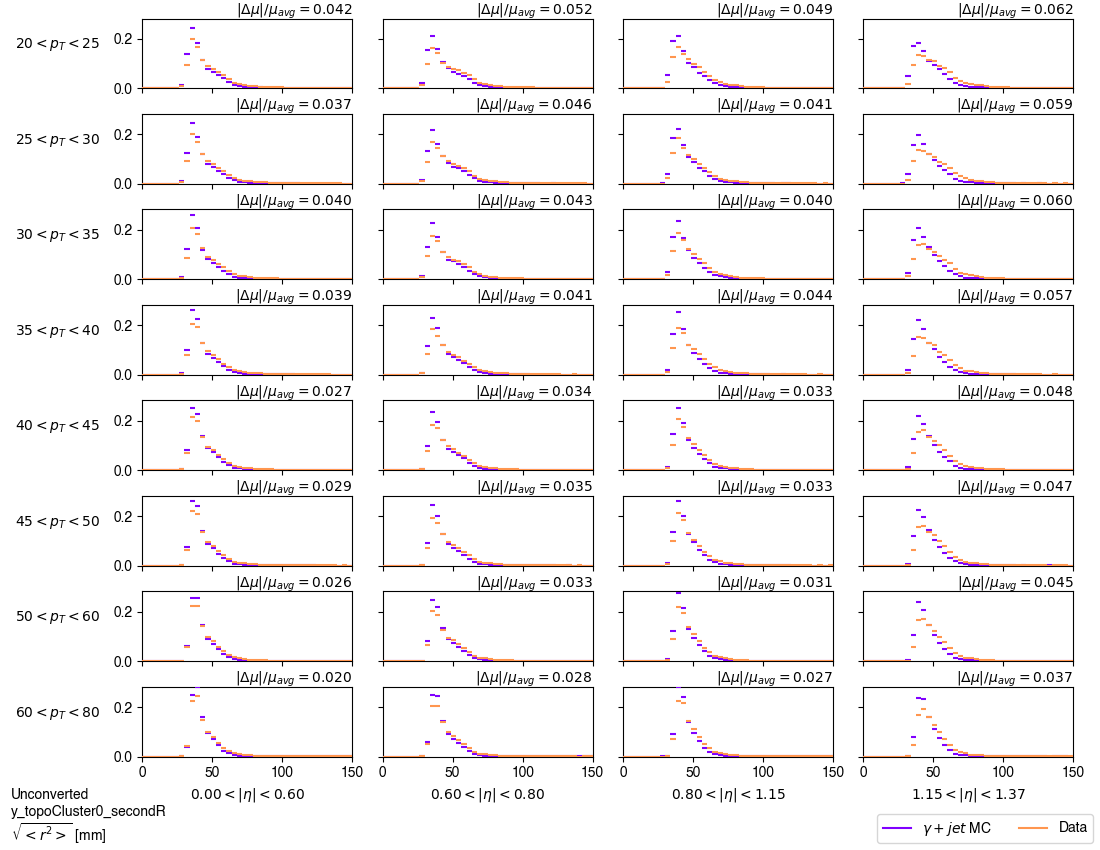
\includegraphics[width=.80\textwidth]{chapters/chapter4_photonID/images/y_topoCluster0_secondR_Unconverted_lowerEta.png}
    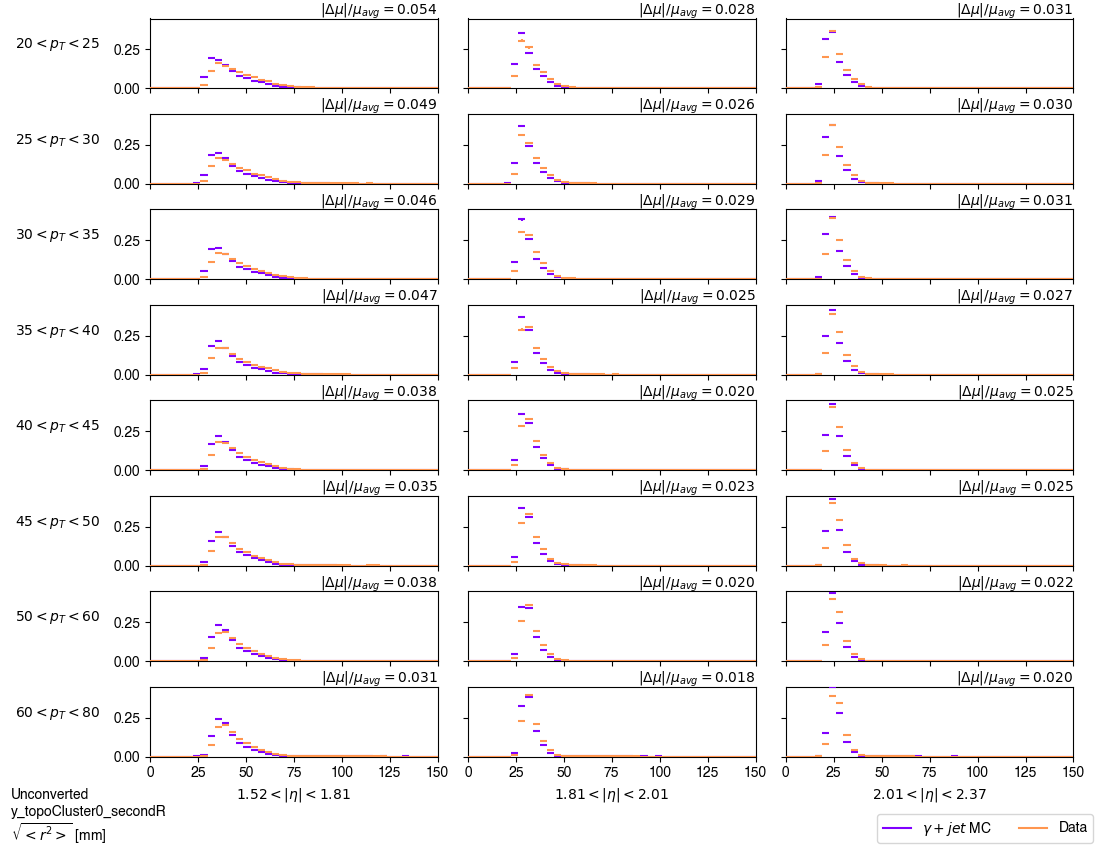
\includegraphics[width=.80\textwidth]{chapters/chapter4_photonID/images/y_topoCluster0_secondR_Unconverted_upperEta.png}
    \caption{Data-MC comparison for the semi-major axis in width ($\sqrt{r^2}$).}
\end{figure}
% TODO: split these figs?

\noindent\textbf{Correlations}\\
\indent Checking the correlations of variables is important for several reasons. First, highly correlated variables do not bring new information, and thus are not useful for adding additional cuts on. Also, it is paramount that any variables that are incorporated in the menu are not correlated to photon isolation. The correlation between these variables and the shower shape variables and isolation working points is shown in Figure \ref{fig:photonid-corrs}. 
%todo: add plots

\begin{figure}[!thp]
    \centering
    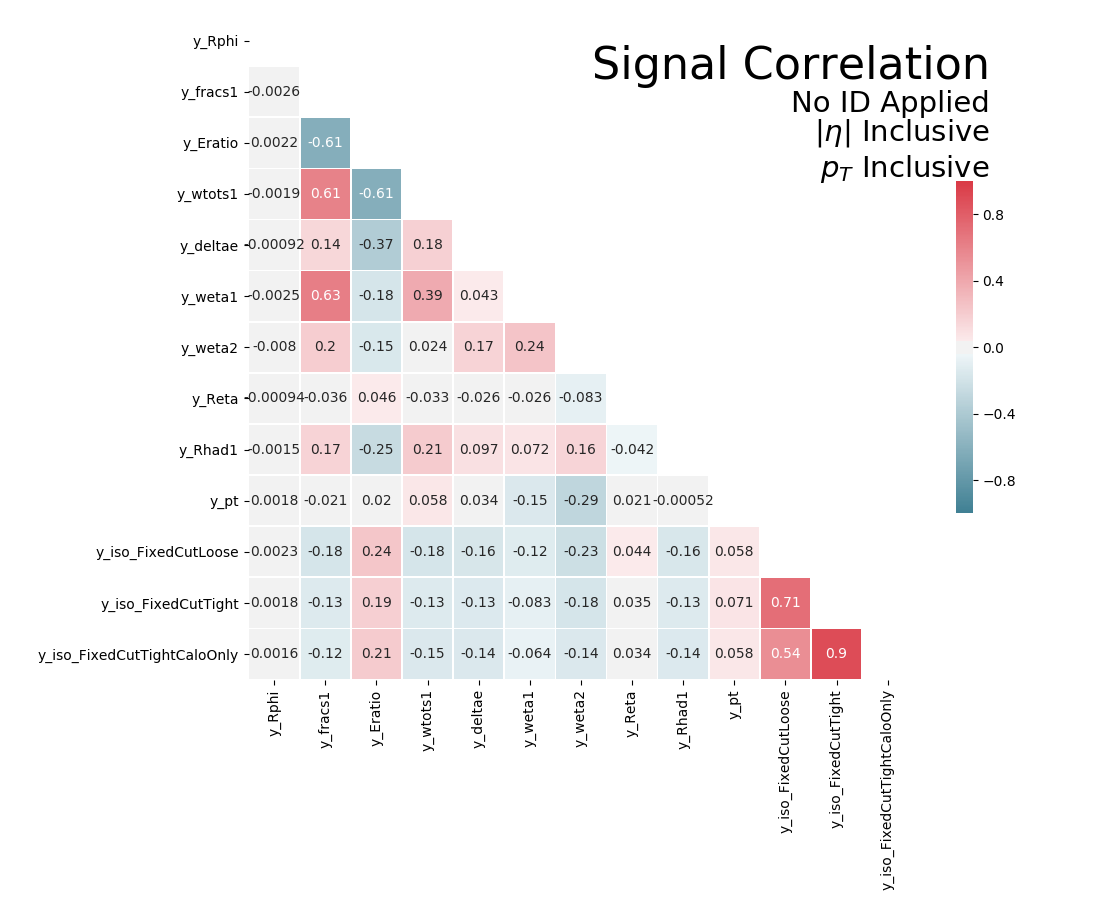
\includegraphics[width=.77\textwidth]{chapters/chapter4_photonID/images/sig_none_corr.png}
    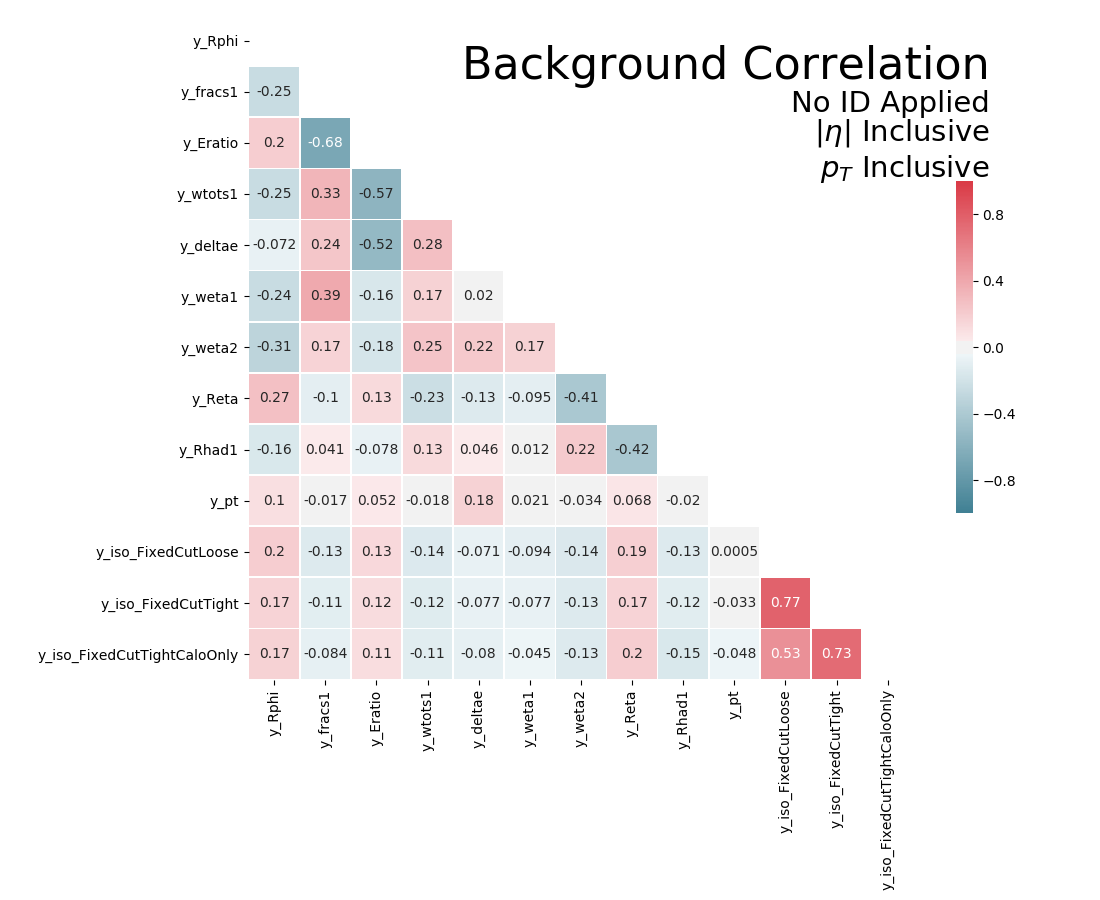
\includegraphics[width=.77\textwidth]{chapters/chapter4_photonID/images/bkg_none_corr.png}
    \caption{Correlation values between the shower shape variables, topological cluster variables, and isolation working points.}
    \label{fig:photonid-corrs}
\end{figure}
% TODO: split these figs?

\subsection{Incorporating into Menu}

The topological cluster variables were added to the existing shower shape variable-based menu. The cut-based approach is reoptimized including the new variables, and new cuts are derived in each $\eta$-\pt bin. To compare improvement across bins, a figure of merit is defined, the improvement in background rejection for the same signal efficiency as the current photon identification menu. In formulaic terms:

\begin{align}
    Z &= \frac{(1-\epsilon_{bkg,i}) - (1-\epsilon_{bkg,0})}{(1-\epsilon_{bkg,0})} = \frac{\epsilon_{bkg,0} - \epsilon_{bkg,i}}{1-\epsilon_{bkg,0}}
    \label{eqn:improvement-metric}
\end{align}

For figure of merit $Z$, and background efficiency $\epsilon_{bkg}$ (thus, background rejection is $(1-\epsilon_{bkg}$), where index $i$ indicates the reoptimized menu, and index $0$ indicates the original menu. This value is calculated bin-wise in $\eta$-\pt and shown in Figure ADD FIG. In principle, adding additional variables to a cut-based method should only improve optimization if the search over possible cut values is exhaustive. However, in several bins, worse performance is found by incorporating new variables. This can be the result of two causes:
\begin{itemize}
    \item In a high dimensional space, such a grid search becomes computationally prohibitive, so a Genetic Algorithm\footnote{The Genetic Algorithm used is a standard method implemented in \texttt{TMVA}, and the details of implementation can be found in Reference \cite{TMVA}.} \cite{genetic-algo} is used to find an approximate solution, and thus increasing dimensionality has the possibility to find local minima, and thus suboptimal solutions.
    \item Statistical fluctuations. As standard, models are trained on an orthogonal subset of events than they are evaluated on, and statistical fluctuations in these samples can influence reported gain, particularly in low stats bins. Figure \ref{fig:photonid-events} shows the number of signal and background events in each $\eta$-\pt bin.
\end{itemize}

\begin{figure}[!thp]
    \centering
    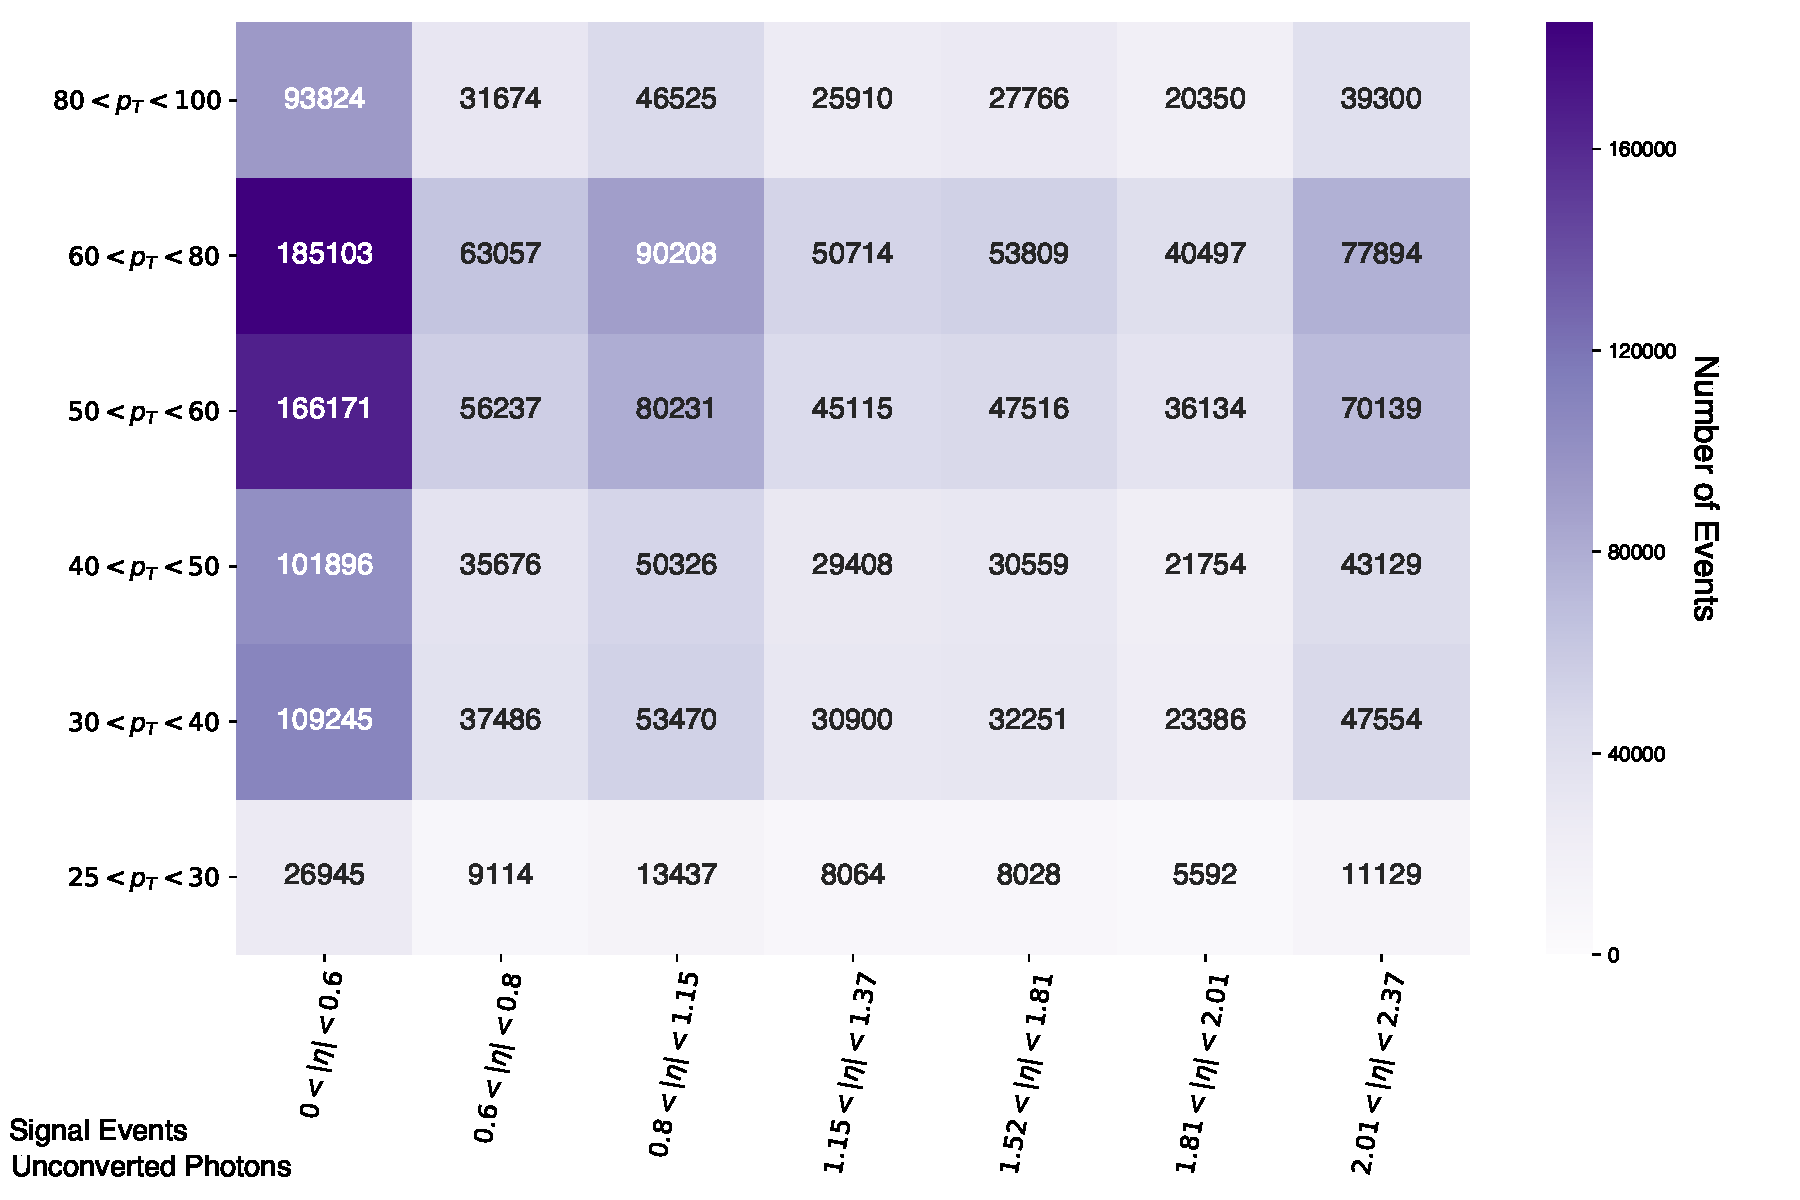
\includegraphics[width=.85\textwidth]{chapters/chapter4_photonID/images/sig_events.pdf}
    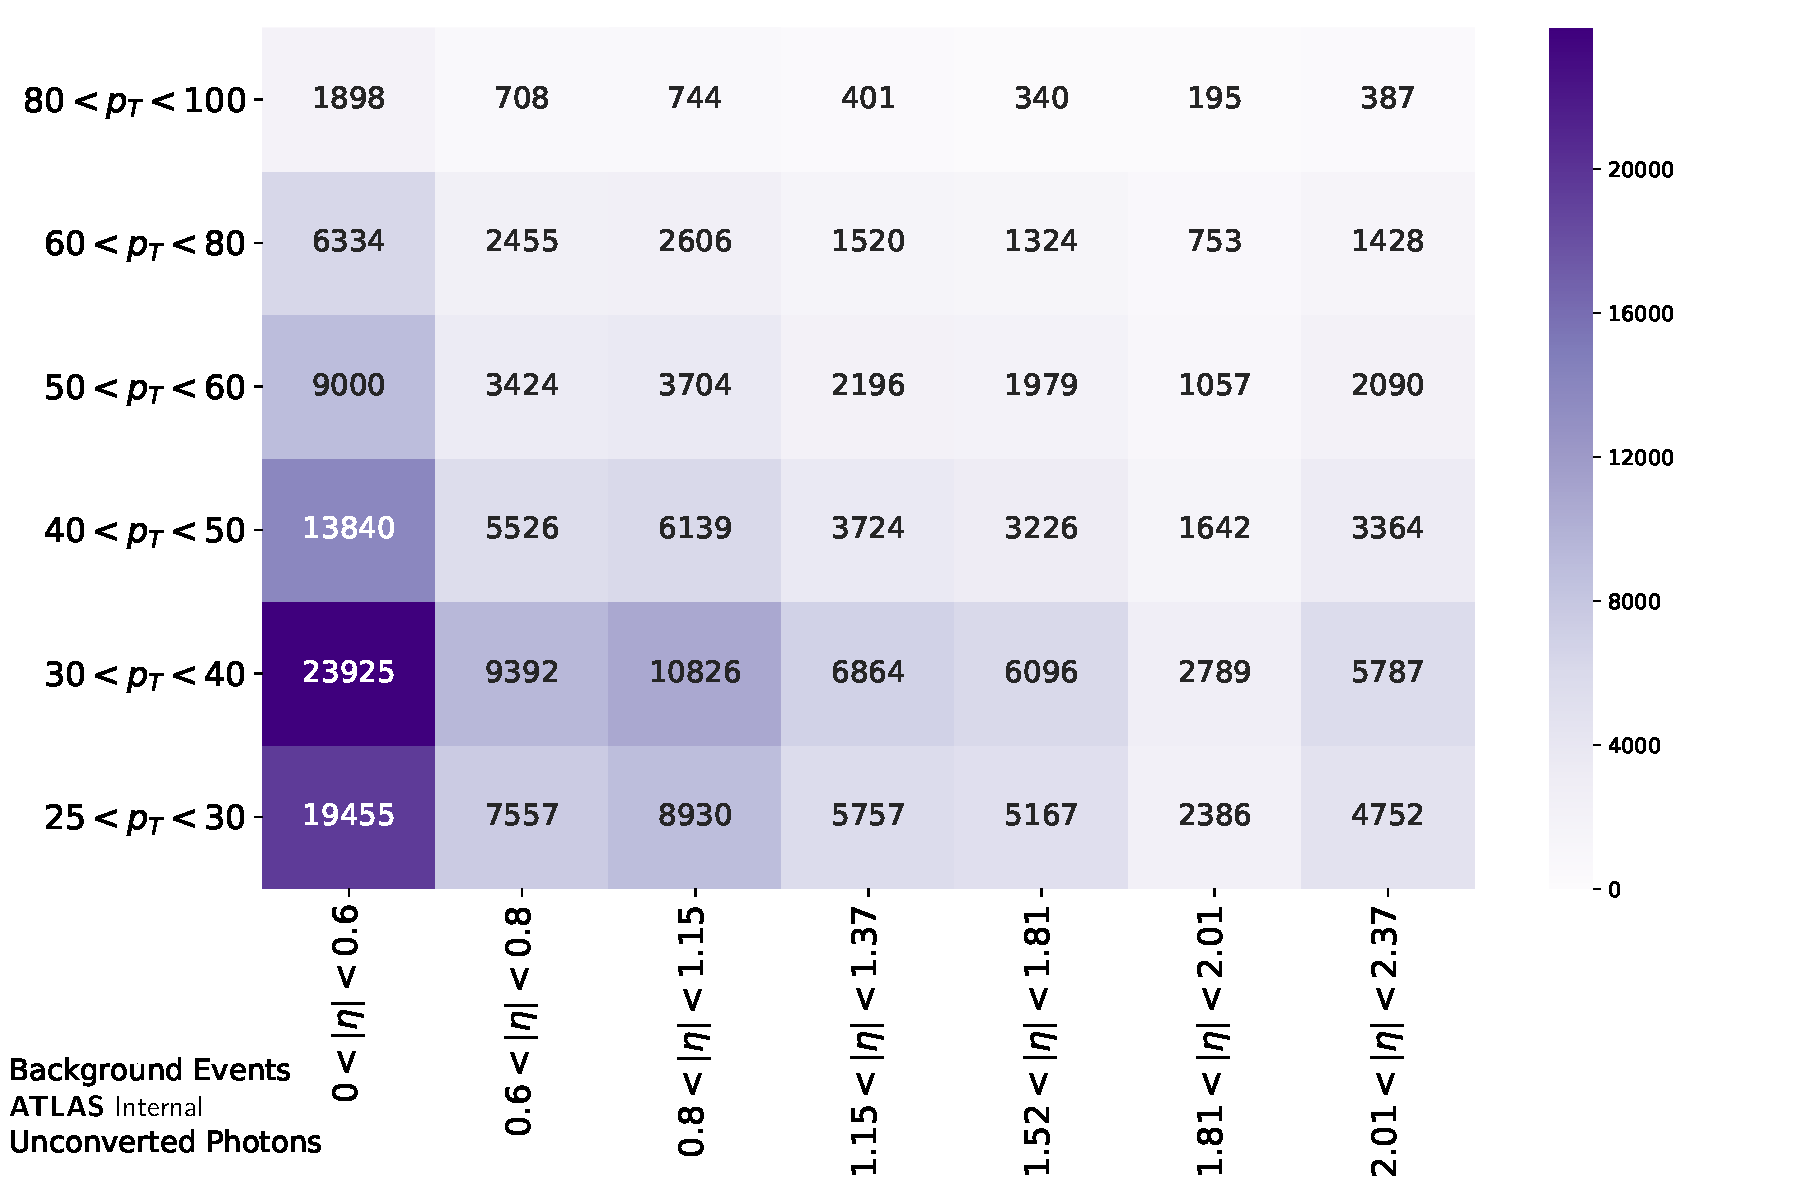
\includegraphics[width=.85\textwidth]{chapters/chapter4_photonID/images/bkg_events.pdf}
    \caption[Number of training events for in each $\eta$-\pt bin for the signal $\gamma$+jets sample, and the background jet fakes sample]{Number of training events for in each $\eta$-\pt bin for the signal $\gamma$+jets sample (top), and the background jet fakes sample (bottom). The preselection described in Section \ref{sec:photon-id-samples} is used.}
    \label{fig:photonid-events}
\end{figure}


\section{Multivariate Analysis Techniques}

The current photon identification working points are defined by a rectangular cuts method. Cut optimization is performed through a 9-dimensional scan over the shower shape variables. In order to better reject background, a multivariate approach to defining these working points has been investigated. These methods are outlined in detail in Appendix \ref{app:MVA}, and the following sections will discuss the improvements brought to photon identification through implementing them.

\subsection{Boosted Decision Tree}

A gradient boosted \gls{BDT} was employed as an alternative classification algorithm. A major problem in training these \glspl{BDT} was the lack of background training statistics when segmenting into $\eta$-\pt bins. To navigate this problem, rather than training an independent model for each $\eta$-\pt bin, \pt inclusive models were trained. As shown in Figure \ref{fig:photonid-corrs}, the input variables have low correlation to \pt, and thus this does not bias the model.




As a baseline, the \gls{BDT} is compared to the cut-based photon identification menu, using the same figure of merit defined in Equation \ref{eqn:improvement-metric}, where the efficiency denoted $i$ represents the \gls{BDT} model, and the efficiency denoted $0$ represents the current cut-based model.


\subsection{Neural Network}